\documentclass[11pt,a4paper]{article}
\usepackage[T1]{fontenc}
\usepackage[utf8]{inputenc}
\usepackage{geometry}
\usepackage{graphicx}
\usepackage[table]{xcolor}
\usepackage{colortbl}
\usepackage{hyperref}
\usepackage{longtable}
\usepackage{array}
\usepackage{tabularx}
\usepackage{booktabs}
\usepackage{enumitem}
\usepackage{caption}
\usepackage{subcaption}
\usepackage{listings}
% Define a lightweight JSON language for listings to avoid package error
\lstdefinelanguage{json}{
  basicstyle=\ttfamily\small,
  showstringspaces=false,
  morestring=[b]",
  stringstyle=\color{brown},
  literate={true}{{{\color{blue}true}}}{4}
       {false}{{{\color{blue}false}}}{5}
       {null}{{{\color{magenta}null}}}{4}
       {\{}{{\{}}{1}
       {\}}{{\}}}{1}
       {[}{{[}}{1}
       {]}{{]}}{1},
}
\usepackage{float}
\usepackage{fancyhdr}
\usepackage{microtype}
\usepackage{tikz}
\usepackage{tcolorbox}
\usetikzlibrary{positioning,arrows.meta,shadows.blur}
\geometry{margin=1in}
\hypersetup{colorlinks=true,linkcolor=blue,urlcolor=blue,citecolor=blue}
% Brand colors
\definecolor{headerbg}{HTML}{F6F8FA}
\definecolor{headerfg}{HTML}{24292E}
\definecolor{themelight}{HTML}{2F81F7}
\definecolor{tablebg}{HTML}{F6F8FA}
\definecolor{tablerule}{gray}{0.85}
\graphicspath{{../assets/screenshots/}}
\setlength{\parskip}{0.6em}
\setlength{\parindent}{0pt}
\setlength{\emergencystretch}{2em}

% Removed repeating header; use plain style
\pagestyle{plain}
\captionsetup[figure]{labelfont=bf,font=small}

\author{Pujith Sai Kumar Korlepara\\IIT Bombay (ID: 25M0787)\\Email: \href{mailto:pujith@cse.iitb.ac.in}{pujith@cse.iitb.ac.in} / \href{mailto:pujith22.sde@gmail.com}{pujith22.sde@gmail.com}\\GitHub: \href{https://github.com/pujith22}{pujith22}\\LinkedIn: \href{https://www.linkedin.com/in/pujith22}{in/pujith22}\\Portfolio: \href{https://www.cse.iitb.ac.in/~pujith}{cse.iitb.ac.in/~pujith}}
\date{\today}

\begin{document}
\begin{tcolorbox}[colback=headerbg,colframe=themelight,boxrule=0.8pt,arc=4pt,width=\textwidth]
\centering
{\LARGE \textbf{Persistent Key-Value Store}}\\[0.35em]
{\large Architectural \& API Reference}\\[0.9em]
Pujith Sai Kumar Korlepara\\
IIT Bombay (ID: 25M0787)\\
Email: \href{mailto:pujith@cse.iitb.ac.in}{pujith@cse.iitb.ac.in} / \href{mailto:pujith22.sde@gmail.com}{pujith22.sde@gmail.com}\\
GitHub: \href{https://github.com/pujith22}{pujith22} \quad LinkedIn: \href{https://www.linkedin.com/in/pujith22}{in/pujith22}\\
Portfolio: \href{https://www.cse.iitb.ac.in/~pujith}{cse.iitb.ac.in/~pujith}
\end{tcolorbox}

\textbf{GitHub Repository:} \href{https://github.com/pujith22/persistent-key-value-store}{https://github.com/pujith22/persistent-key-value-store}

\section{Purpose}
A C++17 HTTP service providing a persistent key-value cache backed by PostgreSQL. It exposes a JSON-centric REST API for CRUD and bulk operations while maintaining latency via an inline in-memory write-through cache. Startup fails fast if persistence cannot be reached, enforcing durability guarantees.

\section{High-Level Architecture}
\begin{figure}[H]
  \centering
  % Width adjusted to 95% to remain readable and fit with Purpose on the same page
  \resizebox{1.0\linewidth}{!}{%
  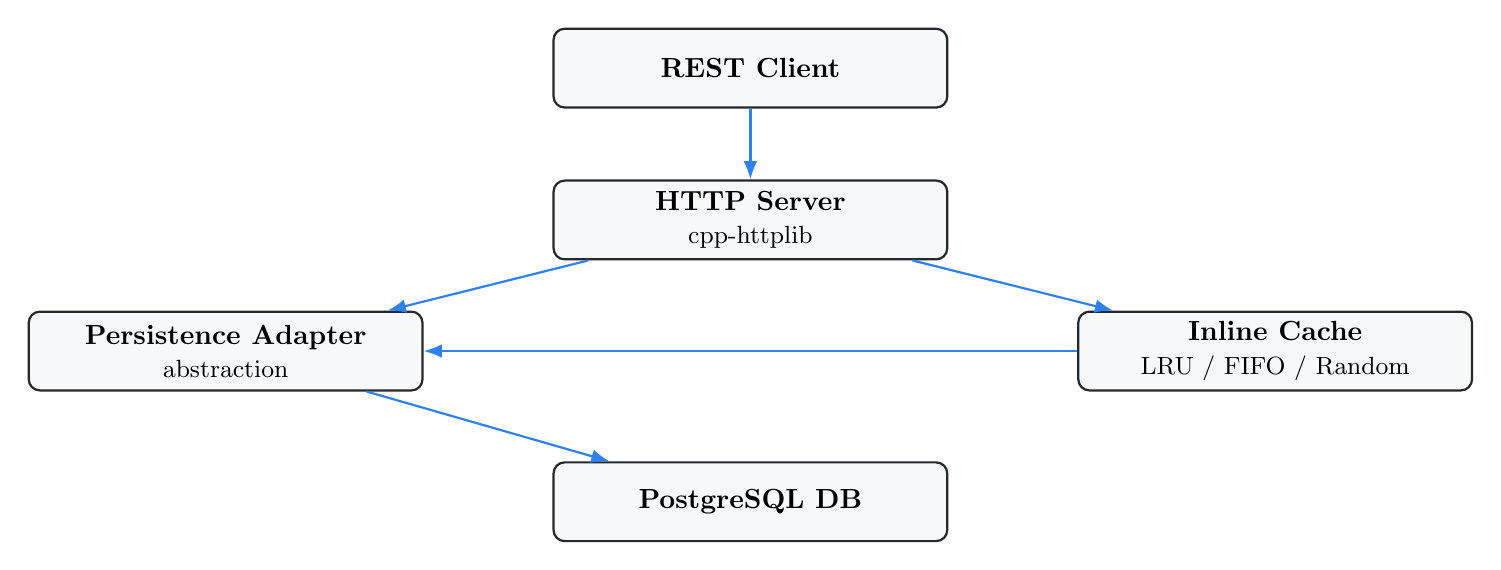
\begin{tikzpicture}[
      scale=1.0,
      node distance=9mm,
      box/.style={draw=headerfg,rounded corners,fill=headerbg,thick,align=center,minimum width=5cm,minimum height=1cm},
      db/.style={draw=headerfg,rounded corners,fill=headerbg,thick,align=center,minimum width=5cm,minimum height=1cm},
      arr/.style={-Latex,thick,draw=themelight}
    ]
    \node[box] (client) {\textbf{REST Client}};
    \node[box, below=of client] (server) {\textbf{HTTP Server}\\\small cpp-httplib};
    \node[box, below right=of server, xshift=10mm] (cache) {\textbf{Inline Cache}\\\small LRU / FIFO / Random};
    \node[box, below left=of server, xshift=-10mm] (adapter) {\textbf{Persistence Adapter}\\\small abstraction};
    \node[db, below=14mm of $(cache)!0.5!(adapter)$] (db) {\textbf{PostgreSQL DB}};

    \draw[arr] (client) -- (server);
    \draw[arr] (server) -- (cache);
    \draw[arr] (server) -- (adapter);
    \draw[arr] (cache) -- (adapter);
    \draw[arr] (adapter) -- (db);
  \end{tikzpicture}}
  \caption{Compact layered architecture: request flow across server, cache, and persistence.}
\end{figure}

% Postman API Collection (moved below Purpose + Architecture)
\section{Postman API Collection}
An interactive Postman collection is published for quick exploration and manual testing of the API surface. You can import it directly via the shared workspace URL below or by copying the JSON specification.

\begin{tcolorbox}[colback=headerbg,colframe=themelight,boxrule=0.6pt,arc=3pt]
	\textbf{Shared Collection URL:} \href{https://www.postman.com/altimetry-architect-63208177/persistent-key-value-server-public/collection/f47ai0l/persistent-key-value-server?action=share&creator=18466773}{Postman Workspace Link}
\end{tcolorbox}

\noindent The local development server (see \texttt{main\_server.cpp}) binds to host \texttt{localhost} on port \texttt{2222}. The collection above targets that base URL.

\begin{tcolorbox}[colback=tablebg,colframe=themelight,boxrule=0.3pt,arc=3pt,title=Minimal Postman Collection JSON]
\begingroup\small
\begin{lstlisting}[language=json,basicstyle=\ttfamily\small,breaklines=true,frame=single]
{
  "info": {
    "name": "Persistent Key Value Store API",
    "schema": "https://schema.getpostman.com/json/collection/v2.1.0/collection.json",
    "description": "CRUD, bulk query, transactional update and observability endpoints"
  },
  "item": [
    {"name": "Catalog", "request": {"method": "GET", "url": "http://localhost:2222/"}},
    {"name": "Home", "request": {"method": "GET", "url": "http://localhost:2222/home"}},
    {"name": "Get Key (cache/persist)", "request": {"method": "GET", "url": "http://localhost:2222/get_key/42"}},
    {"name": "Bulk Query", "request": {"method": "PATCH", "header": [{"key": "Content-Type", "value": "application/json"}], "body": {"mode": "raw", "raw": "{\n  \"data\": [1,2,3,4]\n}"}, "url": "http://localhost:2222/bulk_query"}},
    {"name": "Insert", "request": {"method": "POST", "url": "http://localhost:2222/insert/42/alpha"}},
    {"name": "Bulk Update Txn", "request": {"method": "POST", "header": [{"key": "Content-Type", "value": "application/json"}], "body": {"mode": "raw", "raw": "{\n  \"ops\": [\n    { \"type\": \"insert\", \"key\": 7, \"value\": \"seven\" },\n    { \"type\": \"get\", \"key\": 7 },\n    { \"type\": \"update\", \"key\": 7, \"value\": \"SEVEN\" }\n  ]\n}"}, "url": "http://localhost:2222/bulk_update"}},
    {"name": "Delete Key", "request": {"method": "DELETE", "url": "http://localhost:2222/delete_key/42"}},
    {"name": "Update Key", "request": {"method": "PUT", "url": "http://localhost:2222/update_key/42/beta"}},
    {"name": "Health", "request": {"method": "GET", "url": "http://localhost:2222/health"}},
    {"name": "Metrics", "request": {"method": "GET", "url": "http://localhost:2222/metrics"}},
    {"name": "Stop (dev only)", "request": {"method": "GET", "url": "http://localhost:2222/stop"}}
  ]
}
\end{lstlisting}
\endgroup
\end{tcolorbox}

\clearpage

\section{Endpoint Catalog}
The service exposes the following HTTP endpoints.

\begin{tcolorbox}[colback=tablebg,colframe=themelight,boxrule=0.7pt,arc=3pt,width=\textwidth]
% Method color badges
\definecolor{getc}{HTML}{1F883D}
\definecolor{postc}{HTML}{0969DA}
\definecolor{patchc}{HTML}{A47500}
\definecolor{putc}{HTML}{8250DF}
\definecolor{delc}{HTML}{CF222E}
\newcommand{\badge}[2]{\begingroup\setlength{\fboxsep}{1pt}\colorbox{#1!15}{\textcolor{#1}{\textbf{\texttt{#2}}}}\endgroup}
\newcommand{\GET}{\badge{getc}{GET}}
\newcommand{\POST}{\badge{postc}{POST}}
\newcommand{\PATCH}{\badge{patchc}{PATCH}}
\newcommand{\PUT}{\badge{putc}{PUT}}
\newcommand{\DELETE}{\badge{delc}{DELETE}}
\renewcommand{\arraystretch}{1.18}
\setlength{\tabcolsep}{6pt}
\arrayrulecolor{tablerule}
\newcommand{\codepath}[1]{\texttt{\detokenize{#1}}}
\begin{tabularx}{\textwidth}{>{\bfseries\raggedright\arraybackslash}p{0.13\linewidth} >{\raggedright\arraybackslash}p{0.35\linewidth} X}
  \cellcolor{themelight}\color{white}\textbf{Method} & \cellcolor{themelight}\color{white}\textbf{Path} & \cellcolor{themelight}\color{white}\textbf{Description} \\
\midrule
\rowcolors{2}{tablebg}{white}
\GET & \codepath{/} & Machine-readable service catalog \\
\GET & \codepath{/home} & Formatted documentation for available routes \\
\GET & \codepath{/get_key/:key_id} & Return the value for the provided numeric key, caching it if not present in cache \\
\PATCH & \codepath{/bulk_query} & Retrieve multiple keys in one request; missing keys noted in response; always returns success with errors appended \\
\POST & \codepath{/insert/:key/:value} & Insert a key/value pair; conflicts return 409 with existing value; write-through to cache and persistence \\
\POST & \codepath{/bulk_update} & Transactional pipeline for create/get/insert/update; rolls back on failure and returns failure response \\
\DELETE & \codepath{/delete_key/:key} & Remove the provided key from both cache and persistence layer \\
\PUT & \codepath{/update_key/:key/:value} & Update an existing key with a new value in both cache and persistence layer \\
\GET & \codepath{/health} & Report service health and uptime \\
\GET & \codepath{/metrics} & Expose cache metrics including hit/miss counts \\
\GET & \codepath{/stop} & Gracefully stop the server (testing/debug only; not for production) \\
\bottomrule
\end{tabularx}
\end{tcolorbox}

\pagebreak
\section{Screenshots}
% Sequential numbering (Figure N, Figure N+1, ...) for each screenshot instead of subfigure labels.
% We avoid subfigure environments and use captionof{figure} inside minipages to increment the figure counter twice.
% Generic pair macro: two large stacked images, each becomes its own numbered figure.
\newcommand{\StackImagePair}[4]{% #1 top file, #2 top caption, #3 bottom file, #4 bottom caption
  \begin{center}
    \begin{minipage}{1.0\textwidth}\centering
      \includegraphics[width=1.0\textwidth]{#1}
      \captionof{figure}{#2}
    \end{minipage}\\[1.0em]
    \begin{minipage}{1.0\textwidth}\centering
      \includegraphics[width=1.0\textwidth]{#3}
      \captionof{figure}{#4}
    \end{minipage}
  \end{center}\clearpage}
% First pair should appear immediately after the header (no float repositioning), so reuse same macro.
\newcommand{\StackImagePairHere}[4]{\StackImagePair{#1}{#2}{#3}{#4}}

\StackImagePairHere{root_end_point.png}{Root endpoint (service catalog)}{home_end_point.png}{Home HTML endpoint}
\StackImagePair{get_key_end_point_cache_hit.png}{Cache hit on get\_key}{get_key_end_point_uncached_key.png}{Hydrating uncached key from persistence}
\StackImagePair{get_key_end_point_key_not_exist.png}{Key not found scenario}{insert_end_point_clean_insert.png}{Successful clean insert}
\StackImagePair{insert_end_point_existing_insert.png}{Insert conflict (409)}{update_key_end_point_on_success.png}{Successful update operation}
\StackImagePair{update_key_end_point_on_key_not_present.png}{Update when key absent (404)}{delete_end_point_on_successful_deletion.png}{Successful deletion (204)}
\StackImagePair{delete_key_end_point_on_non_existent_key.png}{Deletion when key not found}{bulk_query_end_point.png}{Bulk query results with mixed statuses}
\StackImagePair{bulk_update_end_point_success.png}{Bulk update transaction success report}{bulk_update_end_point_on_failure.png}{Bulk update transaction failure and rollback}
\StackImagePair{metrics_end_point.png}{Metrics endpoint showing cache statistics}{health_end_point.png}{Health endpoint with uptime}
\StackImagePair{stop_end_point.png}{Stop endpoint (dev only)}{server_log_on_every_request_response.png}{Structured JSON logging output sample}

% Last single image (odd count)
\begin{figure}[p]\centering
  \includegraphics[width=1.0\textwidth]{server_running_with_custom_cache_eviction_policy.png}
  \caption{Server startup with custom cache eviction policy.}
\end{figure}
\clearpage

% (legacy minipage-based screenshot blocks removed in favor of StackImagePair)


\section{Credits}
Third-party libraries: \href{https://github.com/nlohmann/json}{nlohmann/json} and \href{https://github.com/yhirose/cpp-httplib}{cpp-httplib}. Licensed under MIT (see project LICENSE).

\vfill\centerline{\small Generated on \today\; from live source (server.cpp).}
\end{document}
